

\documentclass{article}
\usepackage{graphicx}
\usepackage{wrapfig}
\usepackage{array}
\usepackage{url}
\usepackage{graphicx}
\usepackage{wrapfig}
\usepackage{float}
\title{Packet Analysis (Chapter4 Case Study)}

\author{Mohsen Tavakoli, Joseph Maan Anayee, Seyi Akinlade, Nima Moradianzadeh}

\begin{document}

\maketitle

\section{Problem description}
In this assignment we aims to analyzing the packet capture and also collect the information from a suspected persons activities.
 
The following questions will help guide your investigation:
• Provide any online aliases or addresses and corresponding account credentials that
may be used by the suspect under investigation.
• Who did Ann communicate with? Provide a list of email addresses and any other
identifying information.
• Extract any transcripts of Ann’s conversations and present them to investigators.
• If Ann transferred or received any files of interest, recover them.
• Are there any indications of Ann’s physical whereabouts? If so, provide supporting
evidence.
Network:
• Internal network: 192.168.30.0/24
• DMZ: 10.30.30.0/24
• The “Internet”: 172.30.1.0/24 [Note that for the purposes of this case study, we are
treating the 172.30.1.0/24 subnet as “the Internet.” In real life, this is a reserved nonreturnable
IP address space.]
Evidence: Investigators provide you with a packet capture from Ann’s home network,
“evidence-packet-analysis.pcap.” They also inform you that in the course of their monitoring,
they have found that Ann’s laptop has the MAC address 00:21:70:4D:4F:AE
\section{Experiment}
\subsection{simulation}
In order to emulate the network of the problem we used GNS3. GNS3 can be used in order to emulating the complex network. Virtual devices and actual devices can be set by this software\cite{amyot2014system}.


\subsection{topology}
In our Backbone model, we used two Cisco c7200 Routers(R1 and R2) and seven virtual machines. Secondly,in this topology, four Cisco Ethernet Switches have been designed to connect the virtual machines to routers.










Users:

\begin{itemize}
	\item Virtual Machine Linux * 7
	\item Microsoft Loopback Ethernet * 2
	\item WireShark to capture the packets between links. 
	\item Wireshark Pcap (protocol Hierarchy).
\end{itemize}





Network Topology:

\begin{figure}[H]
	\begin{center}
		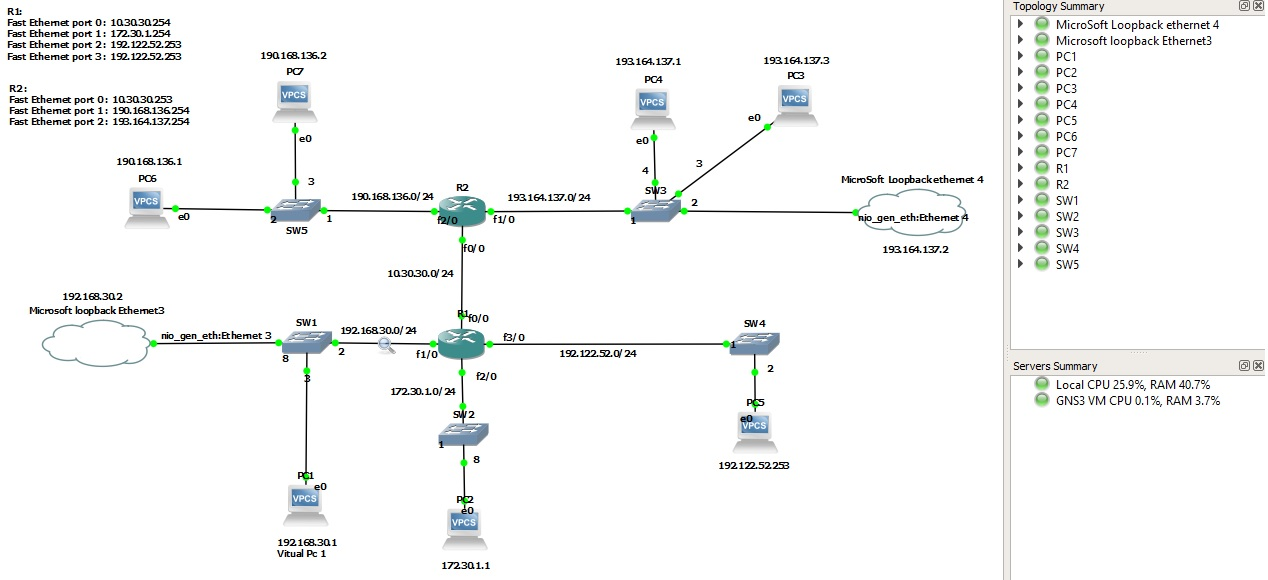
\includegraphics[width=0.6\textwidth]{Topology.jpg}
	\end{center}
	\caption{\small  \newline}
	\label{fig:Prd}
\end{figure}

As you see in this picture you can see that we have 7 virtual pcs and they use DHCP server in order to get IP addresses.\\
How to Install Km-Test Loopback: 

\begin{figure}[H]
	\centering
		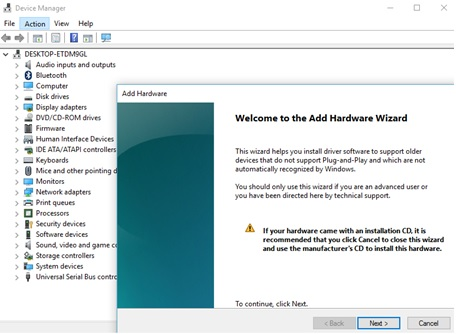
\includegraphics[width=0.48\textwidth]{LoopBackIns1.jpg}
	
	\caption{\small  \newline}
	\label{fig:Prd}
\end{figure}

From device manager we install MS loopback as an additional Network adapter on the computer. Next step is add hardware wizard. Go to install the hardware that I manually select from a list (advance). Under section of network adapters we select KM-Test loopback. After the installation the device is ready to use after one restart of the computer (necessary).

\begin{figure}[H]
	\begin{center}
		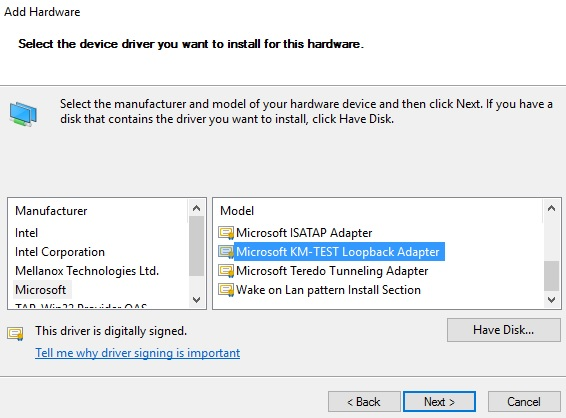
\includegraphics[width=0.48\textwidth]{LoopBackIns2.jpg}
	\end{center}
	\caption{\small  \newline}
	\label{fig:Prd}
\end{figure}


We have 2 Virtual machines connected to the GNS3 using Microsoft Loopback driver Ethernet 3 \& 4.\\


Ethernet 3 – 4:\\
We connected the Ethernet modules to the GNS3 using Cloud in gns3 and add the Loopback Ethernet to the System. And configure (expand here with ip address of each ethernet)(how to configure same as ip network card)(add text)

\begin{figure}[H]
	\begin{center}
		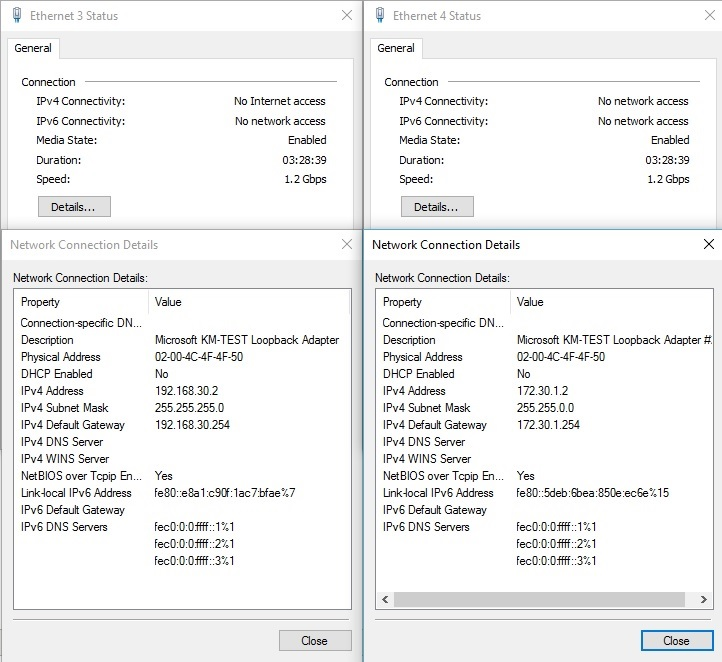
\includegraphics[width=0.48\textwidth]{Ethernet.jpg}
	\end{center}
	\caption{\small  \newline}
	\label{fig:Prd}
\end{figure}


Linus PCs:\\
Explain the Configuration here (contact me if you couldn’t)

\begin{figure}[H]
	\begin{center}
		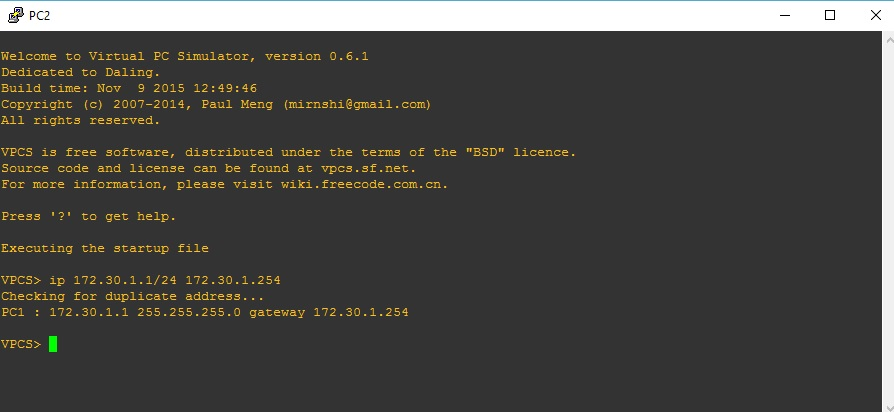
\includegraphics[width=0.48\textwidth]{VPC.jpg}
	\end{center}
	\caption{\small  \newline}
	\label{fig:Prd}
\end{figure}

Ethernet Switches:\\
We configure the switches and grant access to all the ports for future computers.

\begin{figure}[H]
	\begin{center}
		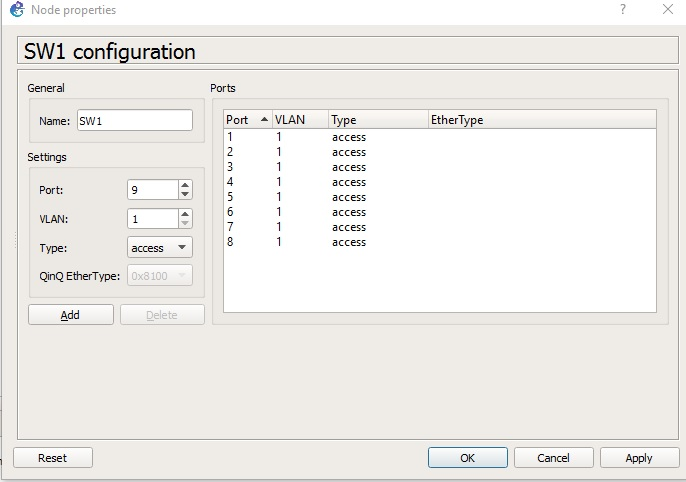
\includegraphics[width=0.48\textwidth]{Switchconf.jpg}
	\end{center}
	\caption{\small  \newline}
	\label{fig:Prd}
\end{figure}

R1 – R2 configurations:\\
Interface Configuration:\\
We start each router and go to enable mode of each router and go to terminal mode:

\begin{figure}[H]
	\begin{center}
		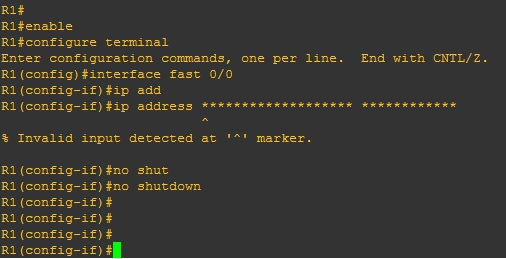
\includegraphics[width=0.48\textwidth]{Terminalconf.jpg}
	\end{center}
	\caption{\small  \newline}
	\label{fig:Prd}
\end{figure}

We configure each terminals.(explain the code)\\

Router RIP Configuration:

\begin{figure}[H]
	\begin{center}
		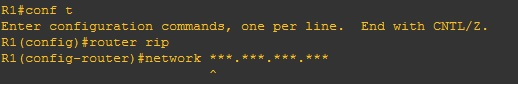
\includegraphics[width=0.48\textwidth]{RouterRip.jpg}
	\end{center}
	\caption{\small  \newline}
	\label{fig:Prd}
\end{figure}

Router 1 Configuration: (do the exact thing for the other router)

\begin{figure}[H]
	\begin{center}
		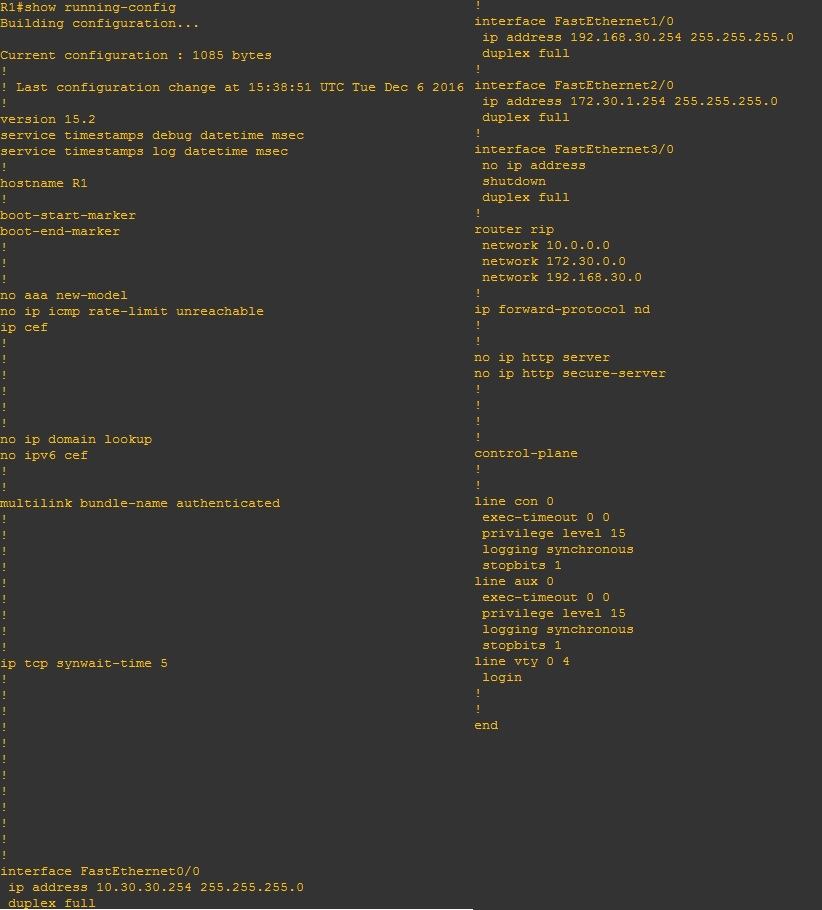
\includegraphics[width=0.48\textwidth]{Routerconfig.jpg}
	\end{center}
	\caption{\small  \newline}
	\label{fig:Prd}
\end{figure}


Wireshark:\\
Explain how we can use Wireshark….

\begin{figure}[H]
	\begin{center}
		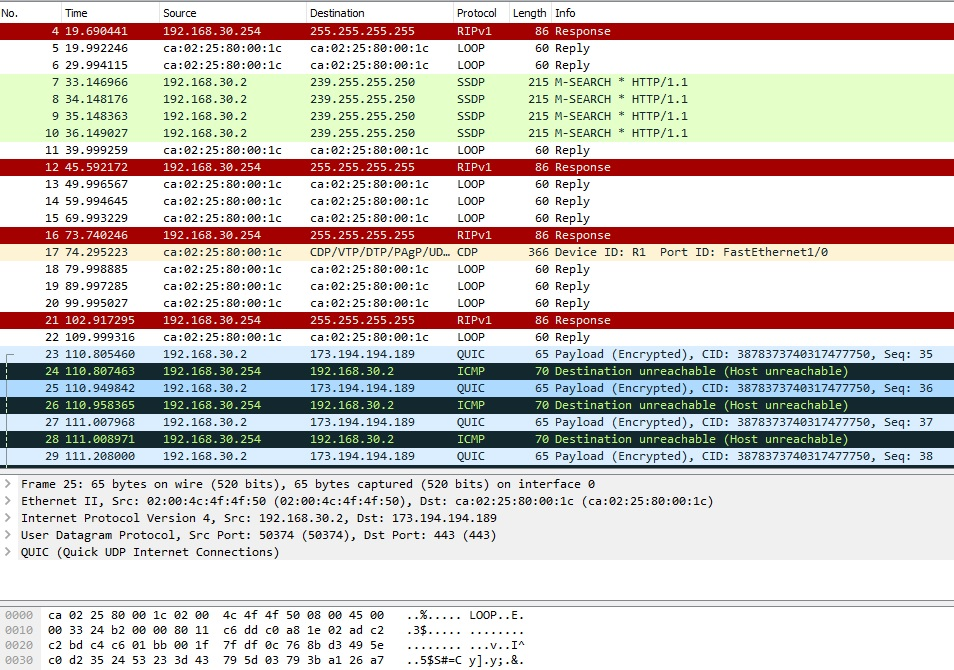
\includegraphics[width=0.48\textwidth]{wireshark.jpg}
	\end{center}
	\caption{ Founded threats by HBGary Responder Pro }
	\label{fig:Prd}
\end{figure}

Protocol Hierarchy:\\
Explain here….


\begin{figure}[H]
	\begin{center}
		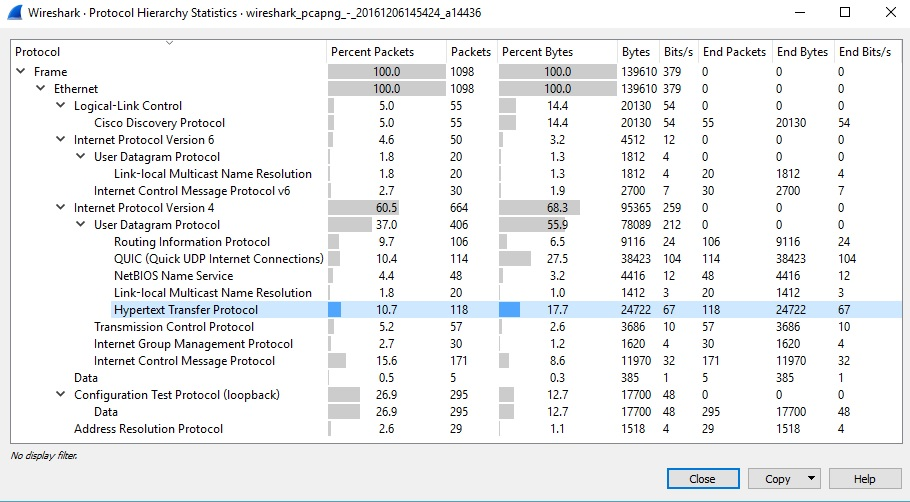
\includegraphics[width=0.48\textwidth]{Hierarchyst.jpg}
	\end{center}
	\caption{\small  \newline}
	\label{fig:Prd}
\end{figure}

\bibliographystyle{ieeetr}
\bibliography{Kent-Case-Study1}
\end{document}
